\documentclass[10pt]{article}
\usepackage{parskip}
\usepackage[margin=1in]{geometry} 
\usepackage{tikz}
\usetikzlibrary{positioning}
\usepackage{amsmath,amsthm,amssymb, graphicx, multicol, array}
\usepackage{enumitem}
\usepackage{xurl}
\usepackage{float}
\usepackage[bb=boondox,bbscaled=.95,cal=boondoxo]{mathalfa}
\usepackage{abstract}
\usepackage{listings}        % for code formatting
\usepackage{xcolor}          % for code syntax colors
\usepackage[hidelinks, breaklinks=true]{hyperref}


% Bibliography
\usepackage[
    backend=biber,
    style=apa,               % APA style (common in marketing)
    sorting=nyt
]{biblatex}
\addbibresource{sources.bib}

% Abstract styling
\renewcommand{\abstractnamefont}{\normalfont\bfseries\large}
\renewcommand{\abstracttextfont}{\normalfont\small}
\setlength{\absleftindent}{0.5in}
\setlength{\absrightindent}{0.5in}

% Code styling
\lstset{
    language=Python,               % change to Python if needed
    basicstyle=\ttfamily\small,
    keywordstyle=\color{blue}\bfseries,
    commentstyle=\color{gray}\itshape,
    stringstyle=\color{red!70!black},
    numbers=left,
    numberstyle=\tiny\color{gray},
    numbersep=8pt,
    frame=single,
    breaklines=true,
    showstringspaces=false,
    tabsize=2,
    captionpos=b
}

\newcommand{\N}{\mathbb{N}}
\newcommand{\Z}{\mathbb{Z}}

\newenvironment{problem}[2][Problem]{\begin{trivlist}
\item[\hskip \labelsep {\bfseries #1}\hskip \labelsep {\bfseries #2.}]}{\end{trivlist}}

\begin{document}

% ── Title ──
\title{Complete Portfolio}
\author{Jakob Sverre Alexandersen\\
GRA4158 Marketing and the Analysis of Experiments and Quasi-Experiments}
\maketitle

% ── Abstract ──
\begin{abstract}
    \noindent
    This portfolio presents solutions to four assignments covering 
    the design and analysis of experiments and quasi-experiments in 
    marketing research. Task~1 estimates the causal effect of digital advertising on purchase conversion using a randomized experiment, addressing non-compliance through IV estimation and assessing ad profitability. Task~2 explores a potential study that examines whether companies can relax their marketing budgets by utilizing more ``normal'' people instead of ``high-maintenance'' influencers to promote their product, and thus attracting more customers.
    Task~3 examines... Task~4 investigates...

    Please note that all code is included in the appendix, and will be referenced throughout the paper. 
\end{abstract}
    

% ── Table of Contents ──
\newpage
\tableofcontents
\newpage

% ══════════════════════════════════════
%   TASKS
% ══════════════════════════════════════

\section{Task 1: The Gen-Z Intern}

\subsection{Non-Compliance Detective}
In order to check for non-compliance, we need to see if the treatment group (test = 1) should see ads (impressions $> 0$), and the control group should NOT see ads (impressions = 0 in practice)

    Since the control group has ``ghost ads'' (hypothetical impressions), non-compliance would be if the control group actually SAW ads. 

\begin{lstlisting}
treatment_group = df[df['test'] == 1]
control_group = df[df['test'] == 0]

treatment_no_exposure = treatment_group[treatment_group['impressions'] == 0]
treatment_with_exposure = treatment_group[treatment_group['impressions'] > 0]

compliance_rate_treatment = len(treatment_with_exposure) / len(treatment_group)
non_compliance_rate = len(treatment_no_exposure) / len(treatment_group)
\end{lstlisting}
\begin{verbatim}
> treatment group size: 25072
> treatment group with impressions > 0 (compliers): 19694
> treatment group with impressions = 0 (non-compliers): 5378
> compliance rate in treatment: 0.7855 (78.55%)
> non-compliance rate: 0.2145 (21.45%)
> control group with 0 ghost impressions: 0.2159017971758665

\end{verbatim}

    The data shows one-sided non-compliance. In the treatment group, 21.45\% were assigned to receive ads but had 0 impressions (the never-takers). The control group shows perfect compliance. The ghost ads system ensures that the control group never actually saw ads. The 21.59\% with 0 ghost impressions simply indicates users who would not have been exposed regardless of assignment. This is \underline{not} two-sided non-compliance because no one in the control group actually received treatment. The full code and outputs for this task is provided in Appendix~\ref{app:task_one}

    We are able to estimate ITT because we have a simple comparison of means by assignment (test = 0 vs test = 1). We cannot observe counterfactual for never-takers who may systematically differ, so we cannot estimate ATE. A naive ATET estimate (comparing those with impressions $> 0 $ in treatment vs. controls) would be biased because never-takers may systematically differ from compliers. Without additional assumptions, ATET is not cleanly identified. LATE is also estimable since using assignment as an instrument for actual exposure estimates effect for compliers. Since we have one-sided non-compliance with perfect compliance in control, LATE = ATET for compliers, which is actually quite informative for managerial decisions. 
\newpage
\subsection{Treatment effect estimates}
The difference in conversion rates between assignment groups is 0.465 percentage points ($p = 0.001$, 95\% CI : [0.2pp, 0.7pp]). This represents the effect of being \textit{assigned} to see ads, regardless of actual exposure. The control group conversion rate was 2.4\% and the treatment group was 2.87\%. 

\begin{lstlisting}
#bin var treatment indicator (actually saw ads)
df['saw_ads'] = ((df['test'] == 1) & (df['impressions'] > 0)).astype(int)

#ITT
itt_control = df[df['test'] == 0]['purchase'].mean()
itt_treatment = df[df['test'] == 1]['purchase'].mean()
itt_effect = itt_treatment - itt_control

print(f'control group conversion rate: {itt_control}')
print(f'treatment group conversion rate: {itt_treatment}\nITT effect: {itt_effect}')

#ITT with regression (for st err)
X_itt = sm.add_constant(df['test'])
model_itt = sm.OLS(df['purchase'], X_itt).fit(cov_type='HC1') #robust SEs 
print(f'regression:\n{model_itt.summary().tables[1]}')
\end{lstlisting}
\begin{verbatim}
> control group conversion rate: 0.024029204107830552
> treatment group conversion rate: 0.028677409061901724
> ITT effect: 0.004648204954071172
> regression:
> ==============================================================================
>                  coef    std err          z      P>|z|      [0.025      0.975]
> ------------------------------------------------------------------------------
> const          0.0240      0.001     24.773      0.000       0.022       0.026
> test           0.0046      0.001      3.245      0.001       0.002       0.007
> ==============================================================================
\end{verbatim}

\textbf{LATE}: Using random assignment as an instrument for actual ad exposure, we estimate the effect of \textit{actually seeing} ads for compliers is 0.59 percentage points ($p = 0.001$, CI: [0.23pp, 0.95pp])

\begin{lstlisting}
#LATE via IV
#instrument: test, endo: saw_ads, outcome: purchase 

df_iv = df[['purchase', 'saw_ads', 'test']].copy()
df_iv['const'] = 1 

iv_model = IV2SLS(
    dependent=df_iv['purchase'],
    exog=df_iv['const'],
    endog=df_iv['saw_ads'],
    instruments=df_iv['test'],
).fit(cov_type='robust')

iv_model.summary
\end{lstlisting}
\newpage 
\begin{verbatim}
> IV-2SLS Estimation Summary
> Dep. Variable:	purchase	R-squared:	0.0015
> Estimator:	IV-2SLS	Adj. R-squared:	0.0015
> No. Observations:	50000	F-statistic:	10.544
> Date:	Wed, Feb 04 2026	P-value (F-stat)	0.0012
> Time:	17:58:29	Distribution:	chi2(1)
> Cov. Estimator:	robust		
> Parameter Estimates
> Parameter	Std. Err.	T-stat	P-value	Lower CI	Upper CI
> const	0.0240	0.0010	24.774	0.0000	0.0221	0.0259
> saw_ads	0.0059	0.0018	3.2471	0.0012	0.0023	0.0095

\end{verbatim}

\textbf{Interpretation}: For every 1,000 users who see the ad, we expect approximately 6 additional conversions compared to not showing ads. The LATE is larger than the ITT because the ITT is diluted by never-takers (users assigned to treatment who never visited the site). 

Note: We do not report an ATET estimate because it would suffer from selection bias, as mentioned in task 1.

\subsection{Impressive Impressions}
\begin{lstlisting}
#create impression bins for strat analysis
df['imp_bins'] = pd.cut(df['impressions'], bins=[-1, 0, 1, 2, 3, 5, 10, 20], labels=['0', '1', '2', '3', '4-5', '6-10', '11+'])

#calc ITT bu imp bin
cate_by_bin = df.groupby(['imp_bins', 'test'])['purchase'].agg(['mean', 'count', 'std']).unstack()
cate_by_bin.columns = ['_'.join(map(str, col)) for col in cate_by_bin.columns] #convert to str before joining
cate_by_bin['ITT'] = cate_by_bin['mean_1'] - cate_by_bin['mean_0']
cate_by_bin['n_total'] = cate_by_bin['count_0'] + cate_by_bin['count_1']

cate_by_bin[['mean_0', 'mean_1', 'ITT', 'n_total']].round(4)
\end{lstlisting}
\begin{verbatim}
>       mean_0	mean_1	ITT   n_total
> imp_bins				
> 0	    0.0000	0.0000	0.0000	10760
> 1	    0.0000	0.0000	0.0000	2932
> 2	    0.0000	0.0000	0.0000	5860
> 3	    0.0000	0.0000	0.0000	7830
> 4-5	0.0000	0.0001	0.0001	14039
> 6-10	0.1302	0.1564	0.0262	8478
> 11+	1.0000	1.0000	0.0000	101
\end{verbatim}
\newpage 
\begin{lstlisting}
    #regression with interaction to test heterogeneity
    #model: purchase ~ test + impressions + test*impressions
        
    df['test_x_imp'] = df['test'] * df['impressions']
    X_interact = sm.add_constant(df[['test', 'impressions', 'test_x_imp']])
    model_interact = sm.OLS(df['purchase'], X_interact).fit(cov_type='HC1')
        
    print(model_interact.summary().tables[1])
    \end{lstlisting}
    \begin{verbatim}
    > ===============================================================================
    >     coef    std err          z      P>|z|      [0.025      0.975]
    > -------------------------------------------------------------------------------
    > const          -0.0533      0.002    -27.571      0.000      -0.057      -0.050
    > test           -0.0067      0.003     -2.420      0.016      -0.012      -0.001
    > impressions     0.0242      0.001     28.343      0.000       0.023       0.026
    > test_x_imp      0.0035      0.001      2.866      0.004       0.001       0.006
    > ===============================================================================
    > - base effect of treatment (at 0 impressions): -0.0066651281558449925
    > - additional effect per impression: 0.003506070910565647
    > - interaction significant? p = 0.004154874372134771
    
\end{verbatim}
The interaction model reveals significant heterogeneity in treatment effects ($p = 0.004 $). The effect of ads increases with the number of impressions: 
\begin{itemize}
    \item 0-5 impressions: near-zero treatment effect (ITT $\approx 0 $)
    \item 6-10 impressions: ITT = 2.62 percentage points, substantially higher than the overall average 
    \item Per-impression effect: each additional impression adds approximately 0.35 percentage points to the treatment effect 
\end{itemize}
This suggests a ``threshold effect'', ads need repeated exposure before influencing purchase behavior. The practical implication is that low-frequency exposure may not be cost-effective; the company should prioritize reaching users with 6+ impressions to maximize ROI. 

These findings supplement our earlier estimates by showing that the overall ITT (0.46pp) and LATE (0.59pp) are \textit{averages across heterogeneous effects}. The true effect for high-exposure users is considerably larger. 
\newpage
\subsection{Is showing ads profitable?}
\begin{lstlisting}
contribution_per_purchase = 200
cost_per_impression = 100 / 1_000

late_effect = 0.0059 
itt_effect = 0.00465

avg_impressions_treatment = df[df['test'] == 1]['impressions'].mean()
avg_impressions_control = df[df['test'] == 0]['impressions'].mean()  # ghost impressions
avg_impressions_compliers = df[(df['test'] == 1) & (df['impressions'] > 0)]['impressions'].mean()
revenue_lift_per_user = itt_effect * contribution_per_purchase
cost_per_user = avg_impressions_treatment * cost_per_impression
net_contribution_per_user_itt = revenue_lift_per_user - cost_per_user
n_treatment = len(df[df['test'] == 1])
total_impressions_treatment = df[df['test'] == 1]['impressions'].sum()

total_revenue_lift = n_treatment * itt_effect * contribution_per_purchase
total_ad_cost = total_impressions_treatment * cost_per_impression
total_net_contribution = total_revenue_lift - total_ad_cost
\end{lstlisting}
\begin{verbatim}
> contribution per purchase: 200 NOK
> cost per impression: 0.1 NOK
> average impressions (treatment): 3.20
> average impressions (compliers only): 4.07
> revenue lift per user: 0.9299999999999999
> ad cost per user: 0.32007418634333124
> net contribution per user: 0.6099258136566688
> ROI: 190.5576393475308
> users in treatment: 25072
> total impressions served: 80249
> expected additional conversions: 116.58479999999999
> total revenue lift: 23316.96 NOK
> total ad cost: 8024.900000000001 NOK
> net contribution: 15292.059999999998 NOK



\end{verbatim}
Yes, the advertising campaign is profitable. Using the ITT estimate, each user assigned to treatment generates a revenue lift of 0.93 NOK ($0.465\%\times 200 \text{NOK} $) at a cost of 0.32 NOK (3.2 impressions $\times 0.10 $ NOK), yielding a \textbf{net contribution of 0.61 NOK per user} and an \textbf{ROI of approximately 190\%}

At the campaign level, the treatment group of $\sim $25k users generated approximately 117 additional conversions, with a total revenue lift of 23,317 NOK against ad costs of 8,025 NOK, for a \textbf{net contribution of 15,292 NOK.}

Sensitivity analysis shows substantial margins of safety; the campaign remains profitable as long as contribution per purchase exceeds 69 NOK (current: 200 NOK). The campaign can tolerate CPM up to 291 NOK before it becomes unprofitable (current: 100 NOK). The treatment effect could fall to $0.16\% $ before breaking even (current: $0.46\% $). All parameters have approximately 66\% margin of safety, indicating that profitability conclusion is robust to measurement uncertainty. 
\begin{figure}[H]
    \centering
    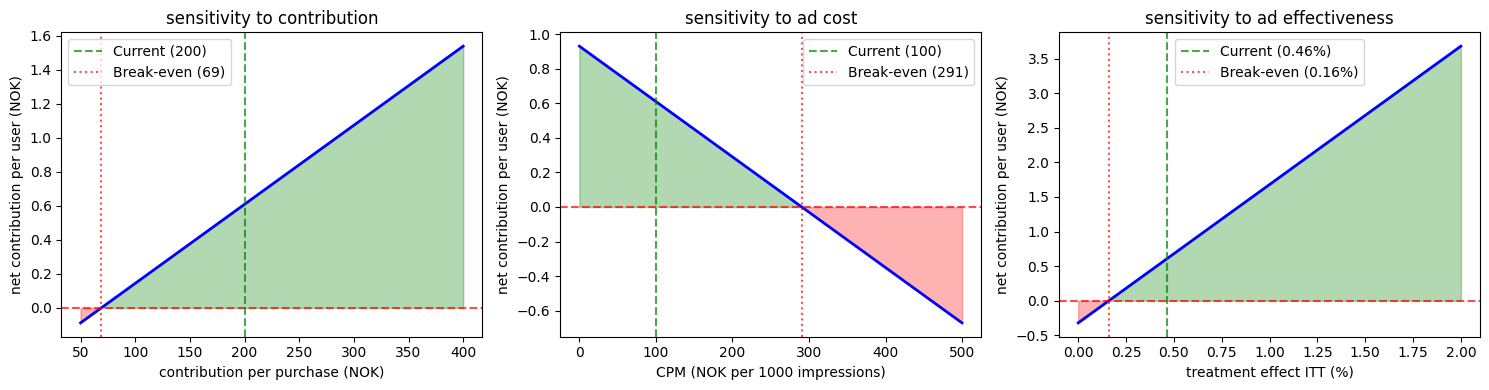
\includegraphics[width=1\textwidth]{image1.png}
\end{figure}

\subsection{Discussion of methods:}
\begin{enumerate}
    \item ITT: We estimated the ITT effect using OLS regression of purchase outcomes on treatment assignment, using heteroskedasticity-consistent standard errors. This approach relies on random assignment, which is satisfied by the experimental design. The primary limitation of the ITT estimate is that it represents a ``diluted'' effect because it includes never-takers who were assigned to treatment but never actually saw ads. Additionally, the linear probability model used for the binary outcome can \textit{in theory} produce predicted probabilities outside the $[0, 1] $ range (although this is rarely problematic for estimating average effects). Alternative approaches include logistic regression (as mentioned in lecture 5), which provide odds-ratios rather than percentage point changes. 
    \item LATE: To account for non-compliance, we estimated the LATE using two-stage least squares with random assignment as an instrument for actual ad exposure. This approach requires four key assumptions: relevance (assignment must affect actual exposure), the exclusion restriction (assignment affects purchase only through ad exposure), monotonicity (no defiers who would only see ads when assigned to control), and independence (random assignment). Our first stage is strong with a compliance difference of 78.5\%, satisfying the relevance condition. 

    The main limitation to LATE is that it identifies the causal effect only for compliers (those who see ads when assigned to treatment and don't see ads when assigned to control). This effect may not generalize to never-takers, whose response to ads we cannot observe. The exclusion restriction is fundamentally untestable and could be violated if merely being part of an experiment affects behavior independently of ad exposure. Alternative approaches include bounds analysis, which relaxes assumptions at the cost of wider intervals, or principal stratification methods. 
    \item CATE: We examined effect heterogeneity by impression level using an interaction model that included treatment, impressions and their product. This approach test whether the treatment effect varies systematically with exposure intensity. The key assumption is that this relationship is linear, which may miss more complex non-linear patterns such as threshold effects or diminishing returns. The ghost ads design is particularly valuable here, as it allows us to compare treatment and control groups at the same hypothetical exposure levels. 
    
    Limitations include the parametric nature of the interaction specification and concerns about multiple comparisons when testing many sub-groups. Small sample sizes at extreme impression levels (the 11+ bin in the code contains only 101 observations) also reduce precision and reliability for those estimates. More flexible alternatives include causal forests or other ML-based methods. 

    Our inference relies on asymptotic approximations with robust standard errors to account for heteroskedasticity, which is particularly important for binary outcomes where variance inherently depends on the mean. With 50k observations, large-sample approximations are generally reliable. However, our standard errors do not account for potential clustering --- if users share devices or households, observations may not be independent, and cluster-robust standard errors would be more appropriate. 
    
    \item SUTVA has two components: no interference between units and no hidden versions of treatment. The first component requires that one user's treatment status does not affect another user's outcome. This could be violated through word-of-mouth (a user who sees the ad might tell a user in the control group about the ad, influencing their purchase decision), shared devices / households, or social network effects. These inference effects would typically cause us to \textit{underestimate} the true ad effect, because some of the treatment ``spills over'' to control. The second component assumes that there is only one version of treatment. In this experiment, users could receive different numbers of impressions, which are effectively different ``doses'' of treatment. Our CATE analysis showed that the treatment effect varies substantially with impression count; users with 6+ impressions showed much larger effects than those with 1-5 impressions. The heterogeneity in treatment intensity means our average estimates (ITT, LATE) mask important variation. The single ``treatment effect'' is actually a weighted average across very different exposure levels. 

    \item The exclusion restriction (for IV/LATE) requires that random assignment affects purchases \textit{only through} actual ad exposure. This could be violated through the Hawthorne effect; if users somehow became aware that they were in an experiment and let it affect their behavior. It could also be affected through the tracking cookie placed for randomization; by itself, it might affect user experience or trigger other platform behaviors that influence purchase. In this experiment, the ghost ads design helps satisfy the exclusion restriction by ensuring the control group has comparable tracking to the treatment group. This is a strength of the experimental design. If the exclusion restriction were to be violated, it would bias the LATE estimate. The direction depends on how the violation affects behavior. 

    \item Monotonicity requires that no user would see ads only when assigned to control. In this design, monotonicity is satisfied by construction; the control group cannot see ads regardless of assignment, and the ghost ads system ensures one-sided non-compliance.

    \item Random assignment appears satisfied by the cookie-based randomization. We could verify this by checking for balance on observable pre-treatment characteristics if such data were available. Without additional covariates in the dataset, we rely on the experimental design description. 

    The most concerning potential violation is interference through word-of-mouth or shared households, which cause us to underestimate the true ad effect. However, in a large-scale digital advertising context with 50,000 users, spillover effects are likely diluted across many social networks, suggesting the bias is probably modest. The heterogeneity in treatment intensity (varying impression) is documented in the CATE analysis rather than being a hidden bias 
\end{enumerate}

\newpage
\section{Task 2: Just Buy This, I Don't Know What Else to Tell You}

\subsection{Introduction \& Research Question}
The relationship between younger consumers and advertising is undergoing a fundamental shift. Adoption of ad-blocking software among young internet users has grown at approximately 40\% year-over-year in the US in 2015 (\cite{sterling2015adblocking}), and eye-tracking research on digital natives reveals that intrusive advertising formats (pop-ups, non-skippable video ads, and content-reorganizing banners) are perceived as deeply annoying and are actively avoided (\cite{fi16040125}). This is not merely a technological trend; it reflects a generational change in how advertising credibility is evaluated. \textcite{DJAFAROVA20171} found that young consumers perceive non-traditional content creators, like bloggers, and YouTubers, as significantly more credible and persuasive than traditional celebrity endorsers or conventional brand advertisements. More recent work confirms that influencer authenticity has a strong positive effect on Gen~Z trust and purchase intentions (\cite{gohil2025influencer}), and that Gen~Z consumers view authentic influencers as ``highly educated friends'' from whom they seek advice, rather than as paid advertisers (\cite{singer2023influencer}).

Given this shift, brands are investing heavily in influencer marketing. However, the question of \textit{what style} of influencer content is most effective remains open. On one end of the spectrum, brands commission polished, high-production influencer partnerships with scripted copy and studio-quality visuals. On the other end, a growing number of creators adopt a raw, casual aesthetic: filming on their phone, speaking without a script, and using humor that borders on self-deprecating (e.g., ``honestly just buy this, I don't know what else to tell you''). Observational data might suggest that authentic-looking content generates higher engagement, but such observations are heavily confounded: platforms' targeting algorithms amplify content to audiences predicted to engage with it, and users self-select into following creators whose style they prefer. As \textcite{braun2025abtesting} demonstrate, even randomized A/B tests conducted through platform-provided tools suffer from \textit{divergent delivery}, where the algorithm serves different ad variants to systematically different user populations, making it impossible to attribute differences to content alone.

This report proposes an experiment to test the following causal question: \textbf{does casual, authentic-style influencer content cause higher purchase intent than professionally produced influencer content?} The focal treatment effect concerns the \textit{perceived authenticity} of the content style, not the presence or absence of influencer marketing itself. The remainder of this report specifies the independent and dependent variables, discusses the operationalization of the treatment and counterfactual, evaluates alternative experimental designs, and analyzes threats to internal and external validity.

\subsection{Variables and Operationalization}
\subsubsection{Independent Variable}
The theoretical independent variable is content authenticity style; the degree to which influencer content appears spontaneous, unpolished, and genuine versus professionally produced and scripted. This construct is operationalized through two experimental conditions:

The treatment condition presents casual, authentic influencer content. Concretely, this is a short video (approximately 30--60 seconds) filmed on a smartphone in a natural setting (e.g., the influencer's home), with informal language, minimal editing, and a conversational tone. The influencer speaks directly to the camera without a visible script, and the product endorsement is embedded in casual commentary.

The control condition presents professional, polished influencer content. This is a video of identical length featuring \textit{the same influencer} promoting \textit{the same product}, but filmed with studio lighting, high-quality audio, scripted copy, and polished editing resembling a traditional sponsored post.
\newpage 
\subsubsection{Counterfactual and the Compound Treatment Problem}
The choice to use the same influencer and the same product across both conditions is a deliberate design decision to avoid the \textit{compound treatment problem}. As discussed in the course, a compound treatment arises when the experimental manipulation unintentionally varies multiple factors simultaneously. If we compared influencer~A (casual) with influencer~B (professional), any observed difference could be attributed to the person, their audience, their delivery style, or the content format, and not solely to authenticity. By holding the influencer and product constant, the manipulation isolates the content style dimension as cleanly as possible.

The counterfactual is an \textit{explicit alternative} rather than the absence of content. This is appropriate because the research question concerns the \textit{relative} effectiveness of two content strategies, not whether influencer content works at all. A ``no content'' control group would answer a different question and would not provide actionable guidance for the business decision at hand.
\subsubsection{Dependent Variable}
The primary dependent variable is purchase intent, which captures the consumer's likelihood of purchasing the promoted product after viewing the content. In the proposed field setting, this is operationalized through behavioral measures recorded via a unique tracked link embedded in each post. Each experimental condition (casual and professional) contains a distinct UTM-tagged or affiliate URL pointing to the product page, allowing the researcher to attribute downstream behavior (click-through, add-to-cart, and conversion) to the specific content variant that generated it. These revealed-preference measures avoid the well-documented gap between stated intentions and actual purchasing behavior, providing a direct read on how content style influences real consumer decisions. Were the experiment instead conducted in a lab, the dependent variable would be measured using a validated 7-point Likert scale (e.g., ``How likely are you to purchase this product?'') supplemented by a hypothetical willingness-to-pay measure. Although they are useful proxies, they are inherently less actionable than observed behavior.

\subsubsection{Challenges in Manipulation and Measurement}

Two key challenges deserve attention. First, regarding manipulation effectiveness: casual content may vary not only perceived authenticity but also perceived humor, effort, or production quality. In a lab setting, this would be verified through explicit manipulation checks where participants rate perceived authenticity, humor, and production quality. In the proposed field setting, however, such self-report measures are unavailable. The researcher cannot directly confirm that authenticity is the primary dimension being varied, which means the field experiment tests the \textit{bundle} of features that distinguish casual from professional content rather than authenticity in isolation. This is a genuine limitation of the field design and one of the strongest arguments for a complementary lab study to probe the underlying mechanism.

Second, regarding measurement of the DV: although the tracked link provides a clean attribution path from content to behavior, the resulting measures are noisy. A single click does not imply genuine purchase intent, and conversion rates in influencer campaigns are typically low, requiring large sample sizes to detect modest effects. The link also introduces a minor demand artifact: users who notice the tracked URL may behave differently than they would with an organic link, though this concern is mitigated by the fact that UTM parameters and affiliate links are standard practice in influencer content and are unlikely to be noticeable to most users. Furthermore, behavioral data alone cannot reveal \textit{why} participants acted as they did. The mechanism remains a black box. A lab experiment lets researchers measure not just outcomes but also things that might explain them, like perceived authenticity or trust, but this extra detail comes at the cost of realism. A field study, on the other hand, sacrifices some of that detail but relies on the underlying theory to help make sense of the results.
\newpage 
\subsection{Experimental Design Strategy}

\subsubsection{Between-Subjects Design}

The proposed experiment uses a between-subjects design, in which each participant is randomly assigned to view either the casual or the professional video, but not both. This choice is driven by the nature of the treatment. A within-subjects design, where the same participant views both videos, would be inappropriate for two reasons. First, it would introduce severe \textit{carryover effects}: once a participant has seen the casual version, their reaction to the professional version (or vice versa) would be contaminated by the comparison. Second, it would create strong \textit{demand effects}, as participants would almost certainly infer that the study is comparing the two styles and adjust their responses accordingly. Both threats are discussed extensively in this course as primary concerns for within-subjects designs.

Between-subjects designs eliminate these concerns at the cost of requiring more participants (since each participant provides data for only one condition) and introducing the possibility of pre-existing differences between groups. However, the latter concern is addressed through random assignment, which ensures that (in theory) the two groups are equivalent on all observed and unobserved characteristics. To further strengthen balance on key demographics (age, gender, social media usage frequency), \textit{stratified random assignment} can be employed, randomizing within homogeneous subgroups rather than across the full sample. This is particularly important if we wish to analyze heterogeneous treatment effects across demographic subgroups.

\subsubsection{Lab vs.\ Field Experiment}

\textbf{The Case for a Lab Experiment}

An online lab experiment would offer maximum control over the experimental setting. Each participant could be randomly assigned to view exactly one video within a survey interface, eliminating any interference from platform algorithms. The researcher could include manipulation checks (e.g., ``How authentic did this content feel?'') and mediator scales (perceived trust, perceived effort) alongside the outcome measures. This diagnostic depth is the core advantage of a lab setting: it allows the researcher not only to estimate the treatment effect but also to probe the mechanism through which it operates. The Hawthorne effect is reduced in an online lab relative to a physical lab, since participants complete the task from their own environment.

However, the lab setting carries substantial limitations for this particular research question. Watching an influencer video inside a survey is fundamentally different from encountering it in a social media feed. The social context (likes, comments, share counts, algorithmic placement among other content) is entirely absent, and these cues may moderate the authenticity effect in practice. Casual content may derive part of its appeal from the \textit{contrast} with polished content in the same feed, an effect that disappears in isolation. Furthermore, the dependent variable in a lab must rely on stated purchase intent rather than actual behavior, introducing the well-documented intention--behavior gap. For a research question whose ultimate business relevance lies in real purchasing outcomes, this is a significant sacrifice.

\textbf{The Case for a Field Experiment}

A field experiment, for instance, running an A/B test through Instagram or TikTok's advertising tools, would score highly on the four key features of field experiments identified in this course: real-world context, authenticity of treatment, representativeness of participants, and relevant outcome measures. Participants would encounter the content organically in their social media feed, respond with real behavior (clicks, purchases), and the sample would reflect the actual target population. The ecological validity of such a design would be high, and the dependent variable could be operationalized as actual click-through, add-to-cart, or conversion. These are behavioral measures that directly answer the business question.

The primary internal validity threat of a field experiment is \textit{divergent delivery}. As \textcite{braun2025abtesting} demonstrate, platform A/B testing tools optimize ad delivery based on predicted user-content relevance, meaning that the casual video and the professional video may be served to systematically different user populations. \textcite{gordon2019comparison} reinforce this concern by showing that even with rich individual-level data, selection effects in digital advertising cannot be adequately controlled for after the fact. Additionally, a field experiment does not easily permit manipulation checks, so the researcher cannot directly verify that the treatment operates through perceived authenticity rather than some other channel. Non-compliance is also a concern: not all users assigned to see an ad will actually be exposed, creating one-sided non-compliance that shifts the estimand from ATE to ITT or LATE.

\textbf{Recommended Design: Field Experiment with Mitigation Strategies}

Despite the internal validity threats, the proposed design is a field experiment conducted through a social media platform's advertising infrastructure. The core justification is that the research question is innately about how consumers respond to influencer content \textit{in its natural environment}. Content style effects are likely moderated by the social media context itself; the feed, the social proof signals, the fleeting attention span of scrolling users\footnote{Colloquially referred to as ``brain rot'' by\\Gen~Z users themselves\\named Oxford's Word of the Year for 2024.}, and stripping away that context in a lab would risk studying a phenomenon that does not transfer to the real world. As \textcite{gordon2019comparison} note, the value of field experiments in digital advertising lies precisely in their ability to measure effects on real behavior in real markets.

To address the divergent delivery problem, several mitigation strategies can be employed. First, the brand can configure the platform's ad manager to use \textit{identical audience targeting} for both conditions, restricting delivery to a pre-defined demographic segment (e.g., Instagram users aged 18--30 in a specific geographic region) and disabling algorithmic optimization of creative delivery where the platform allows it. Second, each content variant includes a unique tracked link (UTM-tagged or affiliate URL) to the product page, enabling clean attribution of click-through, add-to-cart, and conversion behavior to the specific condition that generated it. Third, the analysis should report both the intent-to-treat (ITT) estimate and, where exposure data is available, the local average treatment effect (LATE) to account for non-compliance. Fourth, demographic and behavioral covariates collected by the platform (age, gender, usage frequency) can be included in the regression to improve precision and check for balance across conditions. While these measures cannot fully eliminate the divergent delivery concern, they substantially reduce it and make the remaining threat transparent and quantifiable.

The sacrifice relative to a lab experiment is the inability to include manipulation checks or mediator scales. The researcher cannot directly verify that any observed difference operates through perceived authenticity. This limitation should motivate a complementary lab study as a follow-up to probe the mechanism once the field experiment establishes whether a practically meaningful effect exists in the real market.

\subsection{Validity Analysis}

\subsubsection{Threats to Internal Validity}

The most serious internal validity threat is that the platform's algorithm may serve the two ad variants to systematically different audiences, even when targeting parameters are held constant. As \textcite{braun2025abtesting} document, this \textit{divergent delivery} means that any observed difference in outcomes could reflect audience composition rather than content style. The mitigation strategies discussed above, restricting targeting, disabling creative optimization where possible, and checking covariate balance post hoc reduce, but do not fully eliminate this threat. Transparency about residual confounding is essential when interpreting the results.

In a field experiment, not all users assigned to see an ad will actually view it. Some will scroll past before the video loads, others may be served the ad but not attend to it. This one-sided non-compliance means the experiment estimates an intent-to-treat (ITT) effect rather than the average treatment effect on the treated (ATT). Where the platform provides impression-level data, an instrumental-variables approach can recover the local average treatment effect (LATE), but the ITT remains the most policy-relevant estimand for managerial decision-making, since it reflects what happens when the brand \textit{deploys} a given content strategy.

Despite using the same influencer and product across conditions, the casual and professional videos inevitably differ on multiple dimensions, not only authenticity but also humor, perceived effort, visual aesthetics, and potentially video pacing. This means the treatment is not a clean manipulation of a single construct. Unlike in a lab setting, the field experiment does not allow manipulation checks to diagnose which dimensions are driving the effect. This limitation is inherent to the field design and should be acknowledged: the experiment tests the \textit{bundle} of features that constitute casual versus professional content, not authenticity in isolation. Including platform-provided demographic and behavioral covariates in the analysis can partially account for heterogeneous responses, but it cannot tell us \textit{why} the treatment works.

If the same user follows the influencer organically and encounters both the casual and professional content (e.g., through the influencer's own feed alongside the paid ad), treatment contamination may occur. This risk can be reduced by running the two ad variants in non-overlapping time windows or geographic regions, though this introduces potential confounds from temporal or regional differences. Alternatively, the brand can coordinate with the influencer to ensure that only the paid ads are posted during the experimental window.

Behavioral outcomes such as conversion are binary and typically have low base rates in influencer campaigns, meaning the experiment requires a large sample to detect modest effects. A formal power analysis based on historical conversion rates for similar campaigns should be conducted prior to launch. Under-powering the experiment risks a Type~II error that will incorrectly state that content style does not matter.

\subsubsection{Threats to External Validity}

The norms and expectations of content differ across platforms. Casual, ``off-the-cuff'' content is native to TikTok but may feel out of place on LinkedIn or even Instagram. The field experiment is conducted on a single platform, and results should not be generalized to other platforms without replication. However, running the experiment \textit{on} a platform, rather than abstracting away the platform context in a lab, ensures that the estimated effect is valid for at least one real market environment.

The effect of content style likely depends on the product category. Casual, humorous content may be highly effective for ``enjoyment-driven'', low-involvement products (e.g., snacks, fashion accessories) but less so for utilitarian, high-involvement products (e.g., financial services, electronics). The proposed experiment tests a single product category, and the results should not be generalized beyond it without replication.

The effect may depend on the particular influencer's persona. An influencer whose brand is already casual may show a smaller treatment effect than one whose audience expects polished content. While using a single influencer controls for person-level confounds, it limits generalizability. Future replications with multiple influencers would strengthen external validity.


Social media trends evolve rapidly. What reads as ``authentic'' today may feel forced or faux\footnote{Like Wendy's replies on $\mathbb{X}$ (formerly Twitter)} in six months as the casual aesthetic becomes mainstream. The field experiment captures a snapshot of consumer preferences at a particular moment, and its conclusions may have a limited shelf life.

\subsection{Discussion and Conclusion}

This report has proposed an experimental design to test whether casual, authentic-style influencer content causes higher purchase intent than professionally produced influencer content. The focal treatment effect concerns perceived authenticity of the content style, operationalized through two video conditions featuring the same influencer and the same product but differing in production quality, tone, and delivery.

The recommended design is a between-subjects field experiment conducted through a social media platform's advertising infrastructure. This choice prioritizes external validity and behavioral realism; a trade-off that is justified by the nature of the research question. Content style effects are deeply embedded in the social media context: the feed environment, the social proof cues, and the fleeting attention of scrolling users all shape how authenticity is perceived and whether it translates into action. A lab experiment, while offering superior control and the ability to probe mechanisms through manipulation checks, would strip away precisely the contextual factors that make the question business-relevant in the first place.

The field design is not without limitations. The divergent delivery problem documented by \textcite{braun2025abtesting} means that platform algorithms may confound the treatment comparison by serving the two ad variants to systematically different audiences. \textcite{gordon2019comparison} further demonstrate that observational corrections for such selection effects are unreliable. The mitigation strategies proposed like restricting targeting parameters, disabling creative optimization, and checking covariate balance, reduce but do not eliminate this threat. Furthermore, the compound treatment concern remains: without manipulation checks, the experiment cannot isolate \textit{perceived authenticity} from the bundle of features that distinguish casual from professional content. These limitations should motivate a complementary lab study as a follow-up to probe the mechanism once the field experiment establishes whether a practically meaningful effect exists in the real market.

From a practical standpoint, the answer to this research question has direct implications for how brands allocate their influencer marketing budgets. If casual content proves more effective at driving real conversions, the irony is notable: the less brands invest in production, the more they may earn in return \dots at least among the younger consumers who increasingly dictate market trends.


\newpage
\section{Task 3: The Return of the Gen-Z Intern}
In this task, we analyze a promotional campaign where treatment (receiving a discount) was \textit{not} randomized. We have a dataset of 5,000 observations with 20 covariates and must estimate the causal effect of the discount on sales (in USD) using several methods, relying on the conditional independence assumption. All code is provided in Appendix~\ref{app:task_three}.

\subsection{EDA}
First off, we can start by doing some exploratory data analysis to see what we're dealing with: 

\begin{verbatim}
    > Shape: (5000, 22)
    > Treatment distribution: d=0: 2532, d=1: 2468
    > Treatment rate: 0.494
    >
    > Outcome summary by treatment group:
    >     count     mean     std    min     25%     50%     75%     max
    > d
    > 0  2532.0  1587.37  437.91 -328.0  1296.0  1604.0  1889.5  2921.0
    > 1  2468.0  1844.19  411.71  347.0  1563.0  1854.0  2132.0  2984.0
    >
    > Naive difference in means: 256.81

\end{verbatim}

We can observe a nearly 50/50 split in the data, so we don't have to worry about any extreme imbalance in treatment assignment. The naive ATE is 256.81 USD, suggesting that the treated group has substantially higher sales on average. The covariance balance looks surprisingly good, as most differences are tiny. The largest are in $X16 (-0.29)$, $X17 (-0.19)$, $X18 (-0.15)$. These are small but could still confound. The 256.81 USD may still be biased despite the decent balance, we'll learn if that's the case when doing actual estimation.

\subsection{Regression Adjustment}
We estimate the ATE using OLS regression with all 20 covariates and heteroskedasticity-robust standard errors (HC1):

\begin{verbatim}
    > Naive OLS (no controls):   ATE = 256.81, SE = 12.02, p < 0.001
    > Regression adjustment:     ATE =  15.15, SE =  5.79, p = 0.009
    >                            95% CI: [3.81, 26.50]
    >                            R-squared: 0.883
\end{verbatim}

The first thing we (should) take notice of in the output is the massive confounding. The naive estimate drops to 15.15 USD after controlling for covariates! The covariates were heavily confounding the raw comparison. The $R^2 $ is 0.882, telling us that the 20 covariates explain 88.2\% of the sales variance, which is encouraging for the conditional independence assumption: the covariates are highly informative. The main drivers are $X14 (-304)$, $X15 (-134)$, $X7 (+22)$, $X5 (+36)$, and $X20 (-27)$. The treatment effect is still significant at 15.15 USD ($p = 0.009,\, \text{CI: }[3.81, 26.50] $); the discount appears to have a modest positive causal effect. 

However, OLS regression adjustment has known limitations: it imposes a linear functional form, performs variance-weighted estimation, and does not protect against overfitting when the same sample is used for both fitting and inference. 

\newpage 
\subsection{Matching}
\subsubsection{Propensity Score Estimation and Common Support}

We estimate propensity scores using logistic regression on standardized covariates: 

\begin{verbatim}
    > Propensity Score Summary:
    > Control group - mean: 0.26, min: 0.0001, max: 0.99
    > Treated group - mean: 0.73, min: 0.02,   max: 1.00
    >
    > Common support range: [0.02, 0.99]
    > Observations in common support: 5000 / 5000 (100.0%)
\end{verbatim}

\begin{figure}[H]
    \centering
    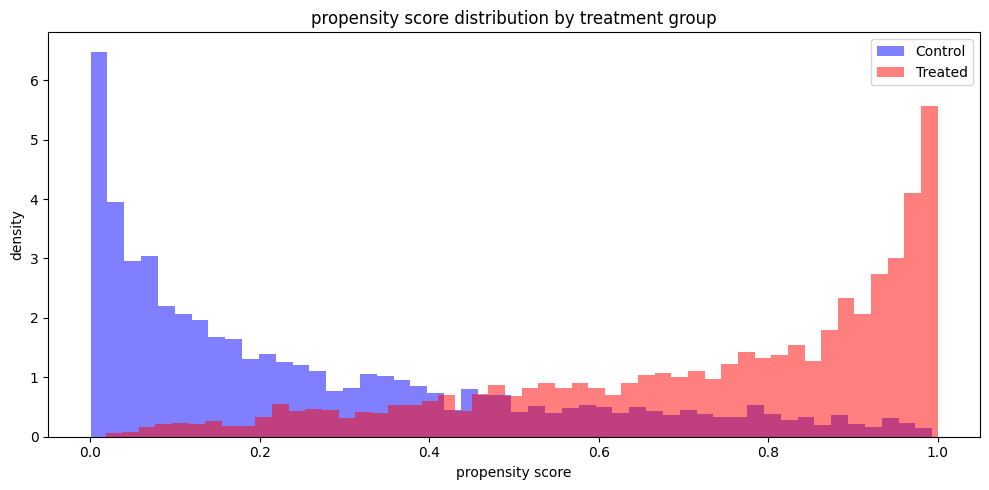
\includegraphics[width=1\textwidth]{2026-03-20-19-01-29.png}
\end{figure}

The figure reveals that the propensity score distributions are heavily separated: control observations cluster near 0 and treated observations cluster near 1. This confirms that the covariates are highly predictive of treatment assignment, consistent with the strong confounding observed earlier. While technically all observations fall within the common support range, the density of the overlap in the middle range ($\sim 0.2 - 0.8 $) is thin relative to the tails. This has direct implications for IPW (discussed below), where extreme propensity scores produce unstable weights. 

\subsubsection{Propensity Score Matching} 

We implement 1:1 nearest-neighbor matching on the propensity score (without replacement). The ATET is $\sim 2.40 $, statistically insignificant (CI: $[\sim 23.70, 18.90] $). Match quality is excellent (mean propensity score distance of 0.0006), and covariance balance is reasonable (mean standardized mean difference of 0.075, max of 0.24). 
\begin{verbatim}
    > Propensity Score Matching (1:1 NN):
    > ATET estimate: -2.40
    > Std err: 10.87
    > 95% CI: [-23.70, 18.90]
    > Mean PS distance: 0.0006
    > Max PS distance:  0.0064
\end{verbatim}


\newpage 
\subsubsection{Mahalanobis Distance Matching}

As an alternative distance measure, we use Mahalanobis distance, which accounts for different variances and correlations between covariates. It is the most common alternative to propensity score matching for multivariate matching. 

\begin{verbatim}
    > Mahalanobis Distance Matching (1:1 NN):
    > ATET estimate: 150.85
    > Std err: 7.66
    > 95% CI: [135.84, 165.87]
    > Mean Mahalanobis distance: 3.45
    > Max Mahalanobis distance:  5.37
\end{verbatim}

The Mahalanobis estimate of 150.85 USD should not be trusted. Covariate balance diagnostics reveal a max standardized mean difference of 1.03, indicating at least one covariate is severely imbalanced after matching. This is the curse of dimensionality: with 20 covariates, Mahalanobis distance must simultaneously minimize discrepancies across all dimensions, resulting in poor matches overall. This illustrates perfectly why propensity score matching is preferred in high-dimensional settings like this one. 
\begin{center}
    \begin{tabular}{lcc}
        \hline
        \textbf{Method} & \textbf{Mean $|$SMD$|$} & \textbf{Max $|$SMD$|$} \\\hline
        PS Matching & 0.075 & 0.242 \\
        Mahalanobis & 0.198 & 1.031 \\\hline
    \end{tabular}
\end{center}

\subsection{Inverse Probability Weighting (IPW)}

Using the IPW estimator with propensity scores clipped to $[0.01,\, 0.99] $ and bootstrap standard errors, we get an ATE of -311.69 USD:

\begin{verbatim}
    > IPW Estimator:
    > ATE estimate: -311.69
    > Bootstrap SE: 81.21
    > 95% CI: [-470.87, -152.51]
    >
    > Weight diagnostics:
    > Treated weights - mean: 1.81, max: 56.29
    > Control weights - mean: 17.44, max: 100.00
\end{verbatim}


This is clearly unreliable. The weight diagnostics reveal the problem: the max control weight hits the clipping ceiling of 100 (1/0.01), and the mean control weight is 17.44, which is far from the ideal $\sim 1 $. As the propensity score plot showed, many control observations have propensity scores near 0, producing extreme inverse weights that dominate the estimate.

\subsection{Augmented Inverse Probability Weighting (AIPW)}

The AIPW estimator combines propensity scores weighting with outcome regression, using a linear regression outcome model and logistic regression propensity model: 

\begin{verbatim}
    > AIPW Estimator (Linear + Logistic):
    > ATE estimate: 18.85
    > Bootstrap SE: 8.42
    > 95% CI: [2.34, 35.35]
\end{verbatim}

The ATE is 18.85 USD (SE = 8.42, CI: $[2.34,\, 35.35] $), close to the regression adjustment estimate (15.15). This is expected: when the outcome model is well-specified, the IPW correction term becomes small, and the estimator is primarily driven by the regression component. This is the double robustness property. 

However, our AIPW implementation does not use cross-fitting, meaning the same observations are used to fit both nuisance models and estimate the treatment effect. This can introduce overfitting bias. 

\subsection{Double ML}

DML addresses the two key challenges of using ML in causal inference: regularization bias (via orthogonalization, based on the Frisch-Waugh-Lovell theorem) and overfitting bias (via 5-fold cross-fitting). We explore three ML algorithms for both the outcome and treatment models: 

\begin{verbatim}
    > DML Summary:
    > ML Method                  ATE      SE     95% CI
    > ---------------------------------------------------------
    > Lasso                     1.00    6.00    [-10.77, 12.77]
    > Random Forest             1.00    5.83    [-10.42, 12.42]
    > Gradient Boosting         1.00    5.94    [-10.65, 12.65]
\end{verbatim}

All three converge to ATE $\sim 1.00 $ USD, which is statistically insignificant. The convergence across fundamentally different ML methods (linear regularized, ensemble bagging, ensemble boosting) provides strong evidence that the result is robust to model choice. 

\subsection{Comparison and Discussion}

\begin{center}
    \begin{tabular}{|c|c|c|c|}
        \hline 
        \textbf{Method} & \textbf{ATE (USD)} & \textbf{Significant?} & \textbf{Trust level}\\\hline 
        Naive (no controls) & 256.81 & Yes & None (confounded)\\\hline 
        Regression adj. & 15.15 & Yes ($p = 0.009 $) & Moderate\\\hline 
        PS Matching & -2.40 & No & Moderate\\\hline 
        Mahalanobis & 150.85 & Yes & Low (bad balance)\\\hline 
        IPW & -311.69 & Yes & None (extreme weights)\\\hline 
        AIPW & 18.85 & Yes ($p < 0.05 $) & Moderate-high\\\hline 
        DML (Lasso) & 1 & No ($p = 0.87 $) & High\\\hline 
        DML (Random Forest) & 1 & No ($p = 0.87 $) & High\\\hline 
        DML (Gradient Boost) & 1 & No ($p = 0.87 $) & High\\\hline 
    \end{tabular}
\end{center}
\subsubsection{Why do the estimates differ?}

The estimates split into two groups: methods without cross-fitting (OLS and AIPW) suggest a modest significant effect of 15-19 USD, while methods with cross-fitting (DML) or nonparametric approaches (PS matching) find a near-zero, insignificant effect of -2 to 1 USD. This pattern is consistent with overfitting bias. DML's cross-fitting explicitly breaks the correlation between prediction errors and the outcome's random errors.

The Mahalanobis estimate (150.85 USD) is an outlier driven by poor matching quality in 20 dimensions, while IPW (-311.69 USD) is dominated by extreme inverse probability weights caused by the separated propensity score distributions. 

\subsubsection{Which estimates do we trust the most?}

DML is the most methodologically rigorous estimator in our comparison: 
\begin{itemize}
    \item It addresses regularization bias through orthogonalization (the Frisch-Waugh-Lovell principle), ensuring that shrinkage in the ML models does not propagate into the treatment effect estimates. 
    \item It addresses overfitting bias through 5-fold cross-fitting, ensuring that predictions are independent of the estimation sample. 
    \item It allows non-linear confounding through flexible ML, relaxing the linearity assumption that OLS regression imposes. 
    \item All three ML algorithms converge to the same estimate, demonstrating robustness to model choice. 
\end{itemize}
The PS matching result (-2.40 USD, insignificant) corroborates the DML finding, despite using a completely different methodology. 

\subsubsection{Assumptions and limitations}
All methods in this analysis rely on the \textit{conditional independence assumptions}: the potential outcomes are independent of treatment conditional on the covariates. If there exist unobserved confounders that influence both treatment assignment and sales, all estimates are biased. The high $R^2 $ (0.883) is reassuring; the 20 covariates explain the vast majority of outcome variation, but it does not guarantee that the selection mechanism is fully captured. 

Additionally, the separated propensity score distributions indicate that the treated and control groups occupy somewhat different regions of the covariate space. While common support technically holds, the thin overlap in the middle range means that some estimates rely on comparisons between units that are not closely comparable, particularly for IPW which assigns extreme weights to observations in low-density regions. 

\subsubsection{Recommendation to the marketing manager}
Based on our analysis, and particularly the DML estimates which we consider most trustworthy, the discount campaign likely has no meaningful causal effect on sales. The naive difference of 257 USD was almost entirely driven by selection effects: customers who received discounts were systematically different from those that did not, and these differences (and not the discount itself) explain the higher sales. 

We recommend the manager not assume that discounts drive incremental revenue based on this observational data. To obtain a definitive answer, we recommend conducting a randomized experiment where discounts are assigned randomly to a subset of customers. This would eliminate confounding by design and provide an unbiased estimate of the discount's true effect. If randomization is infeasible, the company should at minimum collect and control for all variables that influence both discount targeting and purchasing behavior. 


\newpage
\section{Task 4: Title Here}

\subsection{Subtask 4a}
Your content here...

% ══════════════════════════════════════
%   REFERENCES
% ══════════════════════════════════════

\newpage
\printbibliography[title={References}]

% ══════════════════════════════════════
%   APPENDIX
% ══════════════════════════════════════

\newpage
\appendix
\section{Code}
\subsection{Task 1 Code}
\label{app:task_one}
\begin{lstlisting}
import pandas as pd
import numpy as np 
import statsmodels.api as sm
import matplotlib.pyplot as plt 
from linearmodels.iv import IV2SLS
    
pd.set_option('display.max_columns', None)
df = pd.read_csv('CaseData2026.csv', delimiter=';')

treatment_group = df[df['test'] == 1]
control_group = df[df['test'] == 0]

treatment_no_exposure = treatment_group[treatment_group['impressions'] == 0]
treatment_with_exposure = treatment_group[treatment_group['impressions'] > 0]

compliance_rate_treatment = len(treatment_with_exposure) / len(treatment_group)
non_compliance_rate = len(treatment_no_exposure) / len(treatment_group)

print(f"treatment group size: {len(treatment_group)}")
print(f"treatment group with impressions > 0 (compliers): {len(treatment_with_exposure)}")
print(f"treatment group with impressions = 0 (non-compliers): {len(treatment_no_exposure)}")
print(f"compliance rate in treatment: {compliance_rate_treatment:.4f} ({compliance_rate_treatment*100:.2f}%)")
print(f"non-compliance rate: {non_compliance_rate:.4f} ({non_compliance_rate*100:.2f}%)")


control_no_exposure = control_group[control_group['impressions'] == 0]
print(f'control group with 0 ghost impressions: {len(control_no_exposure) / len(control_group)}')
\end{lstlisting}
\begin{verbatim}
    > treatment group size: 25072
    > treatment group with impressions > 0 (compliers): 19694
    > treatment group with impressions = 0 (non-compliers): 5378
    > compliance rate in treatment: 0.7855 (78.55%)
    > non-compliance rate: 0.2145 (21.45%)
    > control group with 0 ghost impressions: 0.2159017971758665
\end{verbatim}
\newpage 
\begin{lstlisting}
#bin var treatment indicator (actually saw ads)
df['saw_ads'] = ((df['test'] == 1) & (df['impressions'] > 0)).astype(int)

#ITT
itt_control = df[df['test'] == 0]['purchase'].mean()
itt_treatment = df[df['test'] == 1]['purchase'].mean()
itt_effect = itt_treatment - itt_control

print(f'control group conversion rate: {itt_control}')
print(f'treatment group conversion rate: {itt_treatment}\nITT effect: {itt_effect}')

#ITT with regression (for st err)
X_itt = sm.add_constant(df['test'])
model_itt = sm.OLS(df['purchase'], X_itt).fit(cov_type='HC1') #robust SEs 
print(f'regression:\n{model_itt.summary().tables[1]}')
\end{lstlisting}
\begin{verbatim}
> control group conversion rate: 0.024029204107830552
> treatment group conversion rate: 0.028677409061901724
> ITT effect: 0.004648204954071172
> regression:
> ==============================================================================
>                  coef    std err          z      P>|z|      [0.025      0.975]
> ------------------------------------------------------------------------------
> const          0.0240      0.001     24.773      0.000       0.022       0.026
> test           0.0046      0.001      3.245      0.001       0.002       0.007
> ==============================================================================
\end{verbatim}
\begin{lstlisting}
#LATE via IV
#instrument: test, endo: saw_ads, outcome: purchase 

df_iv = df[['purchase', 'saw_ads', 'test']].copy()
df_iv['const'] = 1 

iv_model = IV2SLS(
    dependent=df_iv['purchase'],
    exog=df_iv['const'],
    endog=df_iv['saw_ads'],
    instruments=df_iv['test'],
).fit(cov_type='robust')

iv_model.summary
\end{lstlisting}
\begin{verbatim}
> IV-2SLS Estimation Summary
> Dep. Variable:	purchase	R-squared:	0.0015
> Estimator:	IV-2SLS	Adj. R-squared:	0.0015
> No. Observations:	50000	F-statistic:	10.544
> Date:	Wed, Feb 04 2026	P-value (F-stat)	0.0012
> Time:	17:58:29	Distribution:	chi2(1)
> Cov. Estimator:	robust		
> Parameter Estimates
> Parameter	Std. Err.	T-stat	P-value	Lower CI	Upper CI
> const	0.0240	0.0010	24.774	0.0000	0.0221	0.0259
> saw_ads	0.0059	0.0018	3.2471	0.0012	0.0023	0.0095
\end{verbatim}
\newpage 
\begin{lstlisting}
#manual LATE calc: LATE = ITT / compliance rate 
compliance_diff = df[df['test'] == 1]['saw_ads'].mean() - df[df['test'] == 0]['saw_ads'].mean()
late = itt_effect / compliance_diff 

print(f'itt effect: {itt_effect}\ncompliance diff: {compliance_diff}\nLATE: {late}')
\end{lstlisting}
\begin{verbatim}
> itt effect: 0.004648204954071172
> compliance diff: 0.7854977664326739
> LATE: 0.005917527907406948

\end{verbatim}
\begin{lstlisting}
#create impression bins for strat analysis
df['imp_bins'] = pd.cut(df['impressions'], bins=[-1, 0, 1, 2, 3, 5, 10, 20], labels=['0', '1', '2', '3', '4-5', '6-10', '11+'])

#calc ITT bu imp bin
cate_by_bin = df.groupby(['imp_bins', 'test'])['purchase'].agg(['mean', 'count', 'std']).unstack()
cate_by_bin.columns = ['_'.join(map(str, col)) for col in cate_by_bin.columns] #convert to str before joining
cate_by_bin['ITT'] = cate_by_bin['mean_1'] - cate_by_bin['mean_0']
cate_by_bin['n_total'] = cate_by_bin['count_0'] + cate_by_bin['count_1']

cate_by_bin[['mean_0', 'mean_1', 'ITT', 'n_total']].round(4)
\end{lstlisting}
\begin{verbatim}
>     mean_0	mean_1	ITT	n_total
> imp_bins				
> 0	0.0000	0.0000	0.0000	10760
> 1	0.0000	0.0000	0.0000	2932
> 2	0.0000	0.0000	0.0000	5860
> 3	0.0000	0.0000	0.0000	7830
> 4-5	0.0000	0.0001	0.0001	14039
> 6-10	0.1302	0.1564	0.0262	8478
> 11+	1.0000	1.0000	0.0000	101

\end{verbatim}
\newpage 
\begin{lstlisting}
#regression with interaction to test heterogeneity
#model: purchase ~ test + impressions + test*impressions

df['test_x_imp'] = df['test'] * df['impressions']
X_interact = sm.add_constant(df[['test', 'impressions', 'test_x_imp']])
model_interact = sm.OLS(df['purchase'], X_interact).fit(cov_type='HC1')

print(model_interact.summary().tables[1])

print(f"- base effect of treatment (at 0 impressions): {model_interact.params['test']}")
print(f"- additional effect per impression: {model_interact.params['test_x_imp']}")
print(f"- interaction significant? p = {model_interact.pvalues['test_x_imp']}")
\end{lstlisting}
\begin{verbatim}
> ===============================================================================
>                   coef    std err          z      P>|z|      [0.025      0.975]
> -------------------------------------------------------------------------------
> const          -0.0533      0.002    -27.571      0.000      -0.057      -0.050
> test           -0.0067      0.003     -2.420      0.016      -0.012      -0.001
> impressions     0.0242      0.001     28.343      0.000       0.023       0.026
> test_x_imp      0.0035      0.001      2.866      0.004       0.001       0.006
> ===============================================================================
> - base effect of treatment (at 0 impressions): -0.0066651281558449925
> - additional effect per impression: 0.003506070910565647
> - interaction significant? p = 0.004154874372134771

\end{verbatim}
\begin{lstlisting}
contribution_per_purchase = 200
cost_per_impression = 100 / 1_000

late_effect = 0.0059 
itt_effect = 0.00465

avg_impressions_treatment = df[df['test'] == 1]['impressions'].mean()
avg_impressions_control = df[df['test'] == 0]['impressions'].mean()  # ghost impressions
avg_impressions_compliers = df[(df['test'] == 1) & (df['impressions'] > 0)]['impressions'].mean()

print(f"contribution per purchase: {contribution_per_purchase} NOK")
print(f"cost per impression: {cost_per_impression} NOK")
print(f"average impressions (treatment): {avg_impressions_treatment:.2f}")
print(f"average impressions (compliers only): {avg_impressions_compliers:.2f}")
\end{lstlisting}
\begin{verbatim}
> contribution per purchase: 200 NOK
> cost per impression: 0.1 NOK
> average impressions (treatment): 3.20
> average impressions (compliers only): 4.07
\end{verbatim}
\newpage 
\begin{lstlisting}
# method 1: per-user analysis (ITT_based, conservative)

revenue_lift_per_user = itt_effect * contribution_per_purchase
cost_per_user = avg_impressions_treatment * cost_per_impression
net_contribution_per_user_itt = revenue_lift_per_user - cost_per_user

print(f'revenue lift per user: {revenue_lift_per_user}')
print(f'ad cost per user: {cost_per_user}')
print(f'net contribution per user: {net_contribution_per_user_itt}')
print(f'ROI: {(revenue_lift_per_user / cost_per_user - 1) * 100}')
\end{lstlisting}
\begin{verbatim}
> revenue lift per user: 0.9299999999999999
> ad cost per user: 0.32007418634333124
> net contribution per user: 0.6099258136566688
> ROI: 190.5576393475308
\end{verbatim}
\begin{lstlisting}
# method 2: per-complier analysis (LATE-based)

revenue_lift_per_complier = late_effect * contribution_per_purchase
cost_per_complier = avg_impressions_compliers * cost_per_impression
net_contribution_per_complier = revenue_lift_per_complier - cost_per_complier

print(f"revenue lift per complier: {revenue_lift_per_complier} NOK")
print(f"ad cost per complier: {cost_per_complier} NOK")
print(f"net contribution per complier: {net_contribution_per_complier} NOK")
print(f"ROI: {(revenue_lift_per_complier / cost_per_complier - 1) * 100}%")
\end{lstlisting}
\begin{verbatim}
> revenue lift per complier: 1.18 NOK
> ad cost per complier: 0.4074794353610237 NOK
> net contribution per complier: 0.7725205646389762 NOK
> ROI: 189.58516617029494%
\end{verbatim}
\begin{lstlisting}
# campaign-level calc

n_treatment = len(df[df['test'] == 1])
total_impressions_treatment = df[df['test'] == 1]['impressions'].sum()

total_revenue_lift = n_treatment * itt_effect * contribution_per_purchase
total_ad_cost = total_impressions_treatment * cost_per_impression
total_net_contribution = total_revenue_lift - total_ad_cost

print(f"users in treatment: {n_treatment}")
print(f"total impressions served: {total_impressions_treatment}")
print(f"expected additional conversions: {n_treatment * itt_effect}")
print(f"total revenue lift: {total_revenue_lift} NOK")
print(f"total ad cost: {total_ad_cost} NOK")
print(f"net contribution: {total_net_contribution} NOK")
\end{lstlisting}
\begin{verbatim}
> users in treatment: 25072
> total impressions served: 80249
> expected additional conversions: 116.58479999999999
> total revenue lift: 23316.96 NOK
> total ad cost: 8024.900000000001 NOK
> net contribution: 15292.059999999998 NOK
\end{verbatim}
\newpage 
\begin{lstlisting}
# sensitivity analysis

#break-even contribution per purchase
breakeven_contribution = cost_per_user / itt_effect
print(f"break-even contribution per purchase:")
print(f"current: {contribution_per_purchase} NOK")
print(f"break-even: {breakeven_contribution} NOK")
print(f"margin of safety: {(contribution_per_purchase - breakeven_contribution) / contribution_per_purchase * 100}%")

#break-even ad cost per 1000 impressions
breakeven_cpm = (itt_effect * contribution_per_purchase) / avg_impressions_treatment * 1000
print(f"\nbreak-even CPM (cost per 1000 impressions):")
print(f"current: 100 NOK")
print(f"break-even: {breakeven_cpm} NOK")
print(f"margin of safety: {(breakeven_cpm - 100) / breakeven_cpm * 100}%")

#break-even treatment effect
breakeven_effect = cost_per_user / contribution_per_purchase
print(f"\nbreak-even treatment effect (ITT):")
print(f"current: {itt_effect*100}%")
print(f"break-even: {breakeven_effect*100}%")
print(f"margin of safety: {(itt_effect - breakeven_effect) / itt_effect * 100}%")
\end{lstlisting}
\begin{verbatim}
> break-even contribution per purchase:
> current: 200 NOK
> break-even: 68.83315835340457 NOK
> margin of safety: 65.58342082329771%
> 
> break-even CPM (cost per 1000 impressions):
> current: 100 NOK
> break-even: 290.55763934753077 NOK
> margin of safety: 65.58342082329771%
> 
> break-even treatment effect (ITT):
> current: 0.46499999999999997%
> break-even: 0.16003709317166562%
> margin of safety: 65.58342082329771%
\end{verbatim}
\newpage 
\begin{lstlisting}
fig, axes = plt.subplots(1, 3, figsize=(15, 4))

#sensitivity to contribution per purchase
contributions = np.linspace(50, 400, 100)
net_by_contrib = [itt_effect * c - cost_per_user for c in contributions]
axes[0].plot(contributions, net_by_contrib, 'b-', linewidth=2)
axes[0].axhline(y=0, color='red', linestyle='--', alpha=0.7)
axes[0].axvline(x=contribution_per_purchase, color='green', linestyle='--', alpha=0.7, label='Current (200)')
axes[0].axvline(x=breakeven_contribution, color='red', linestyle=':', alpha=0.7, label=f'Break-even ({breakeven_contribution:.0f})')
axes[0].set_xlabel('contribution per purchase (NOK)')
axes[0].set_ylabel('net contribution per user (NOK)')
axes[0].set_title('sensitivity to contribution')
axes[0].legend()
axes[0].fill_between(contributions, net_by_contrib, 0, where=[n > 0 for n in net_by_contrib], alpha=0.3, color='green')
axes[0].fill_between(contributions, net_by_contrib, 0, where=[n < 0 for n in net_by_contrib], alpha=0.3, color='red')

#sensitivity to CPM
cpms = np.linspace(0, 500, 100)
net_by_cpm = [itt_effect * contribution_per_purchase - avg_impressions_treatment * (c/1000) for c in cpms]
axes[1].plot(cpms, net_by_cpm, 'b-', linewidth=2)
axes[1].axhline(y=0, color='red', linestyle='--', alpha=0.7)
axes[1].axvline(x=100, color='green', linestyle='--', alpha=0.7, label='Current (100)')
axes[1].axvline(x=breakeven_cpm, color='red', linestyle=':', alpha=0.7, label=f'Break-even ({breakeven_cpm:.0f})')
axes[1].set_xlabel('CPM (NOK per 1000 impressions)')
axes[1].set_ylabel('net contribution per user (NOK)')
axes[1].set_title('sensitivity to ad cost')
axes[1].legend()
axes[1].fill_between(cpms, net_by_cpm, 0, where=[n > 0 for n in net_by_cpm], alpha=0.3, color='green')
axes[1].fill_between(cpms, net_by_cpm, 0, where=[n < 0 for n in net_by_cpm], alpha=0.3, color='red')

#sensitivity to treatment effect
effects = np.linspace(0, 0.02, 100)
net_by_effect = [e * contribution_per_purchase - cost_per_user for e in effects]
axes[2].plot(effects * 100, net_by_effect, 'b-', linewidth=2)
axes[2].axhline(y=0, color='red', linestyle='--', alpha=0.7)
axes[2].axvline(x=itt_effect*100, color='green', linestyle='--', alpha=0.7, label=f'Current ({itt_effect*100:.2f}%)')
axes[2].axvline(x=breakeven_effect*100, color='red', linestyle=':', alpha=0.7, label=f'Break-even ({breakeven_effect*100:.2f}%)')
axes[2].set_xlabel('treatment effect ITT (%)')
axes[2].set_ylabel('net contribution per user (NOK)')
axes[2].set_title('sensitivity to ad effectiveness')
axes[2].legend()
axes[2].fill_between(effects * 100, net_by_effect, 0, where=[n > 0 for n in net_by_effect], alpha=0.3, color='green')
axes[2].fill_between(effects * 100, net_by_effect, 0, where=[n < 0 for n in net_by_effect], alpha=0.3, color='red')
plt.tight_layout()
plt.show()
\end{lstlisting}
\subsection{Task 3 Code}
\label{app:task_three}
\begin{lstlisting}
    import pandas as pd 
    import numpy as np 
    import statsmodels.api as sm
    import matplotlib.pyplot as plt 
    import seaborn as sns 
    
    pd.set_option('display.max_columns', None)
    df = pd.read_csv('t3.csv')
\end{lstlisting}
\begin{lstlisting}
    print(f'shape: {df.shape}')
    print(f'\ntreatment distribution:\n{df['d'].value_counts()}')
    print(f'\ntreatment rate: {df['d'].mean():.3f}')

    print(f'\noutcome summary by treatment group')
    print(df.groupby('d')['y'].describe().round(2))

    print(f'\nnaive difference in means: {df[df['d']==1]['y'].mean() - df[df['d']==0]['y'].mean():.2f}')

    print(f'\ncovariate balance (mean by treatment group)')
    covariates = [f'X{i}' for i in range(1, 21)]
    balance = df.groupby('d')[covariates].mean().T
    balance.columns = ['Control (d=0)', 'Treated (d=1)']
    balance['Diff'] = balance['Treated (d=1)'] - balance['Control (d=0)']
    print(balance.round(3))
\end{lstlisting}
\begin{verbatim}
    > shape: (5000, 22)
    
    > treatment distribution:
    > d
    > 0    2532
    > 1    2468
    > Name: count, dtype: int64
    > 
    > treatment rate: 0.494
    > 
    > outcome summary by treatment group
    >     count     mean     std    min     25%     50%     75%     max
    > d                                                                
    > 0  2532.0  1587.37  437.91 -328.0  1296.0  1604.0  1889.5  2921.0
    > 1  2468.0  1844.19  411.71  347.0  1563.0  1854.0  2132.0  2984.0
    > 
    > naive difference in means: 256.81
    > 
    > covariate balance (mean by treatment group)
    >      Control (d=0)  Treated (d=1)   Diff
    > X1          24.065         24.059 -0.005
    > X2          14.095         14.110  0.015
    > X3          22.001         22.010  0.009
    > X4          15.763         15.784  0.022
    > X5           0.534          0.542  0.008
    > X6          23.059         23.088  0.029
    > X7          11.346         11.439  0.093
    > X8          10.226         10.459  0.233
    > X9          20.425         20.106 -0.319
    > X10         15.643         14.784 -0.859
    > X11         14.512         13.728 -0.784
    > X12          6.941          5.728 -1.213
    > X13         14.797         13.940 -0.857
    > X14          5.536          4.943 -0.593
    > X15         11.870         11.466 -0.404
    > X16         11.614         11.321 -0.292
    > X17         12.579         12.386 -0.193
    > X18          8.018          7.868 -0.150
    > X19         11.584         11.504 -0.080
    > X20          0.347          0.346 -0.000
\end{verbatim}
\begin{lstlisting}
    covariates = [f'X{i}' for i in range(1, 21)]

    X_naive = sm.add_constant(df[['d']])
    model_naive = sm.OLS(df['y'], X_naive).fit(cov_type='HC1')

    print('naive OLS (no controls)')
    print(f'ATE estimate: {model_naive.params['d']:.2f}')
    print(f'std err: {model_naive.bse['d']:.2f}')
    print(f'p-value: {model_naive.pvalues['d']:.4f}')
    print(f'95% CI: [{model_naive.conf_int().loc['d'][0]:.2f}, {model_naive.conf_int().loc['d'][1]:.2f}]')

    #regression adj (w all covariatse)
    X_adj = sm.add_constant(df[['d'] + covariates])
    model_adj = sm.OLS(df['y'], X_adj).fit(cov_type='HC1')
    print('\nregression adjustment (all 20 covariates)')
    print(f'ATE estimate: {model_adj.params['d']:.2f}')
    print(f'std err: {model_adj.bse['d']:.2f}')
    print(f'p-value: {model_adj.pvalues['d']:.4f}')
    print(f'95% CI: [{model_adj.conf_int().loc['d'][0]:.2f}, {model_adj.conf_int().loc['d'][1]:.2f}]')

    print('\nfull regression summary')
    print(model_adj.summary())
\end{lstlisting}
\begin{verbatim}
    > naive OLS (no controls)
    > ATE estimate: 256.81
    > std err: 12.02
    > p-value: 0.0000
    > 95% CI: [233.26, 280.37]
    > 
    > regression adjustment (all 20 covariates)
    > ATE estimate: 15.15
    > std err: 5.79
    > p-value: 0.0089
    > 95% CI: [3.81, 26.50]
    > 
    > full regression summary
    >                             OLS Regression Results                            
    > ==============================================================================
    > Dep. Variable:                      y   R-squared:                       0.883
    > Model:                            OLS   Adj. R-squared:                  0.882
    > Method:                 Least Squares   F-statistic:                     1485.
    > Date:                Fri, 20 Mar 2026   Prob (F-statistic):               0.00
    > Time:                        18:12:17   Log-Likelihood:                -32219.
    > No. Observations:                5000   AIC:                         6.448e+04
    > Df Residuals:                    4978   BIC:                         6.463e+04
    > Df Model:                          21                                         
    > Covariance Type:                  HC1                                         
    > ==============================================================================
    >                  coef    std err          z      P>|z|      [0.025      0.975]
    > ------------------------------------------------------------------------------
    > const       4697.0456     75.960     61.836      0.000    4548.167    4845.924
    > d             15.1536      5.789      2.618      0.009       3.808      26.500
    > X1             3.0618      1.509      2.029      0.042       0.104       6.020
    > X2            -1.5605      1.809     -0.863      0.388      -5.106       1.985
    > X3             1.3632      1.825      0.747      0.455      -2.215       4.941
    > X4            -2.8476      1.743     -1.634      0.102      -6.264       0.569
    > X5            36.2410      5.662      6.401      0.000      25.144      47.338
    > X6            -1.7214      1.710     -1.007      0.314      -5.073       1.630
    > X7            21.8707      1.795     12.186      0.000      18.353      25.388
    > X8            -1.3171      1.846     -0.714      0.475      -4.934       2.300
    > X9             0.8756      1.800      0.487      0.627      -2.652       4.403
    > X10           -1.3391      1.864     -0.718      0.472      -4.992       2.314
    > X11           -0.1072      3.764     -0.028      0.977      -7.484       7.269
    > X12            1.2723      4.149      0.307      0.759      -6.859       9.404
    > X13           -7.1754      3.710     -1.934      0.053     -14.448       0.097
    > X14         -304.0026      3.630    -83.740      0.000    -311.118    -296.887
    > X15         -133.6610      3.774    -35.414      0.000    -141.058    -126.264
    > X16            0.5139      3.539      0.145      0.885      -6.423       7.450
    > X17            1.5268      3.650      0.418      0.676      -5.628       8.681
    > X18           -1.8884      3.625     -0.521      0.602      -8.993       5.216
    > X19            0.8743      3.360      0.260      0.795      -5.712       7.460
    > X20          -26.9651      5.402     -4.992      0.000     -37.552     -16.378
    > ==============================================================================
    > Omnibus:                        5.993   Durbin-Watson:                   2.018
    > Prob(Omnibus):                  0.050   Jarque-Bera (JB):                6.056
    > Skew:                          -0.067   Prob(JB):                       0.0484
    > Kurtosis:                       3.106   Cond. No.                     2.21e+03
    > ==============================================================================
    > 
    > Notes:
    > [1] Standard Errors are heteroscedasticity robust (HC1)
    > [2] The condition number is large, 2.21e+03. This might indicate that there are
    > strong multicollinearity or other numerical problems.
\end{verbatim}
\begin{lstlisting}
    from sklearn.linear_model import LogisticRegression
    from sklearn.preprocessing import StandardScaler
    import warnings
    warnings.filterwarnings('ignore')

    covariates = [f'X{i}' for i in range(1, 21)]
    X = df[covariates].values
    y_out = df['y'].values
    d = df['d'].values

    #est prop scores
    scaler = StandardScaler()
    X_scaled = scaler.fit_transform(X)

    ps_model = LogisticRegression(max_iter=1000, C=1.0)
    ps_model.fit(X_scaled, d)
    pscore = ps_model.predict_proba(X_scaled)[:, 1]
    df["pscore"] = pscore

    print('propensity score summary')
    print(f'control group - mean: {df[df["d"]==0]["pscore"].mean():.4f}, '
        f'min: {df[df['d']==0]["pscore"].min():.4f}, '
        f'max: {df[df['d']==0]["pscore"].max():.4f}')
    print(f'treated group - mean: {df[df['d']==1]["pscore"].mean():.4f}, '
        f'min: {df[df['d']==1]["pscore"].min():.4f}, '
        f'max: {df[df['d']==1]["pscore"].max():.4f}')

    #common support 
    fig, ax = plt.subplots(1, 1, figsize=(10, 5))
    ax.hist(df[df['d']==0]["pscore"], bins=50, alpha=0.5, label='Control', density=True, color='blue')
    ax.hist(df[df['d']==1]["pscore"], bins=50, alpha=0.5, label='Treated', density=True, color='red')
    ax.set_xlabel('propensity score')
    ax.set_ylabel('density')
    ax.set_title('propensity score distribution by treatment group')
    ax.legend()
    plt.tight_layout()
    plt.show()

    #check overlap region
    common_min = max(df[df['d']==0]["pscore"].min(), df[df['d']==1]["pscore"].min())
    common_max = min(df[df['d']==0]["pscore"].max(), df[df['d']==1]["pscore"].max())
    in_support = ((df["pscore"] >= common_min) & (df["pscore"] <= common_max)).sum()
    print(f'common support range: [{common_min:.4f}, {common_max:.4f}]')
    print(f'observations in common support: {in_support} / {len(df)} ({in_support/len(df)*100:.1f}%)')
\end{lstlisting}
\begin{verbatim}
    > propensity score summary
    > control group - mean: 0.2596, min: 0.0001, max: 0.9934
    > treated group - mean: 0.7337, min: 0.0178, max: 0.9998
\end{verbatim}
\begin{lstlisting}
    from sklearn.neighbors import NearestNeighbors
    from sklearn.linear_model import LogisticRegression
    from sklearn.preprocessing import StandardScaler

    covariates = [f'X{i}' for i in range(1, 21)]
    X = df[covariates].values 
    d = df['d'].values
    y_out = df['y'].values

    scaler = StandardScaler()
    X_scaled = scaler.fit_transform(X)

    #prop score 1:1 nearest neigh
    ps_model = LogisticRegression(max_iter=1000, C=1.0)
    ps_model.fit(X_scaled, d)
    pscore = ps_model.predict_proba(X_scaled)[:, 1]
    df['pscore'] = pscore 

    treated_idx = np.where(d == 1)[0]
    control_idx = np.where(d == 0)[0]

    nn_ps = NearestNeighbors(n_neighbors=1, metric='euclidean')
    nn_ps.fit(pscore[control_idx].reshape(-1, 1))
    distances_ps, indices_ps = nn_ps.kneighbors(pscore[treated_idx].reshape(-1, 1))

    matched_control_idx_ps = control_idx[indices_ps.flatten()]
    att_ps = (y_out[treated_idx] - y_out[matched_control_idx_ps]).mean()
    att_ps_se = (y_out[treated_idx] - y_out[matched_control_idx_ps]).std() / np.sqrt(len(treated_idx))

    print(f'prop score matching (1:1 NN)')
    print(f'ATET estimate: {att_ps}')
    print(f'STD err: {att_ps_se}')
    print(f'95% CI: [{att_ps - 1.96*att_ps_se}, {att_ps + 1.96*att_ps_se}]')
    print(f'mean PS distance: {distances_ps.mean()}')
    print(f'max PS distance: {distances_ps.max()}')

    #support check 
    print(f"control: [{pscore[control_idx].min()}, {pscore[control_idx].max()}]")
    print(f"treated: [{pscore[treated_idx].min()}, {pscore[treated_idx].max()}]")


    #mahalanobis distance 
    cov_matrix = np.cov(X.T)
    cov_inv = np.linalg.inv(cov_matrix)

    nn_mah = NearestNeighbors(n_neighbors=1, metric='mahalanobis', metric_params={'VI' : cov_inv})
    nn_mah.fit(X[control_idx])
    distances_mah, indices_mah = nn_mah.kneighbors(X[treated_idx])

    matched_control_idx_mah = control_idx[indices_mah.flatten()]
    att_mah = (y_out[treated_idx] - y_out[matched_control_idx_mah]).mean()
    att_mah_se = (y_out[treated_idx] - y_out[matched_control_idx_mah]).std() / np.sqrt(len(treated_idx))

    print(f'mahalanobis distance matching (1:1 NN)')
    print(f'ATET estimate: {att_mah}')
    print(f'STD err: {att_mah_se}')
    print(f'95% CI: [{att_mah - 1.96*att_mah_se}, {att_mah + 1.96*att_mah_se}]')
    print(f'mean PS distance: {distances_mah.mean()}')
    print(f'max PS distance: {distances_mah.max()}')

    #matching quality
    print('covariate balance after matching (std mean diff)')
    print(f"{'method':<15} {'mean |SMD|':>12} {'max |SMD|':>12}\n{'-' * 42}")
    for name, matched_ctrl_idx in [('PS Match', matched_control_idx_ps), ('Mahalanobis', matched_control_idx_mah)]:
        smds = []
        for col in covariates: 
            treated_vals = df.loc[treated_idx, col].values 
            control_vals = df.loc[matched_ctrl_idx, col].values 
            pooled_std = np.sqrt((treated_vals.var() + control_vals.var()) / 2)
            if pooled_std > 0: 
                smd = abs(treated_vals.mean() - control_vals.mean()) / pooled_std
            else: 
                smd = 0 
            smds.append(smd)
        print(f'{name:<15} {np.mean(smds):>12.4f} {np.max(smds):>12.4f}')
\end{lstlisting}
\begin{verbatim}
    > prop score matching (1:1 NN)
    > ATET estimate: -2.401539708265802
    > STD err: 10.86664959388228
    > 95% CI: [-23.700172912275068, 18.897093495743466]
    > mean PS distance: 0.0006414092179794127
    > max PS distance: 0.006410513573759324
    > control: [5.235242886897245e-05, 0.9934261103936177]
    > treated: [0.017764962271901913, 0.999836623967377]
    > mahalanobis distance matching (1:1 NN)
    > ATET estimate: 150.85129659643437
    > STD err: 7.660488275297928
    > 95% CI: [135.83673957685042, 165.8658536160183]
    > mean PS distance: 3.4495566129441113
    > max PS distance: 5.372612798799318
    > covariate balance after matching (std mean diff)
    > method            mean |SMD|    max |SMD|
    > ------------------------------------------
    > PS Match              0.0750       0.2424
    > Mahalanobis           0.1976       1.0309
\end{verbatim}
\begin{lstlisting}
    from sklearn.linear_model import LinearRegression, LogisticRegression

    covariates = [f'X{i}' for i in range(1, 21)]
    X = df[covariates].values 
    d = df['d'].values
    y_out = df['y'].values

    scaler = StandardScaler()
    X_scaled = scaler.fit_transform(X)

    #IPW est
    ps_model = LogisticRegression(max_iter=1000, C=1.0)
    ps_model.fit(X_scaled, d)
    pscore = ps_model.predict_proba(X_scaled)[:, 1]

    #clip prop scores to avoid insane weights 
    pscore_clipped = np.clip(pscore, 0.01, 0.99)

    ipw_ate = np.mean(y_out * (d / pscore_clipped - (1 - d) / (1 - pscore_clipped)))

    #bootstrap for std err 
    np.random.seed(42)
    n_boot = 1000
    boot_ipw = []

    for _ in range(n_boot):
        idx = np.random.choice(len(y_out), size=len(y_out), replace=True)
        ps_b = LogisticRegression(max_iter=1000, C=1.0)
        ps_b.fit(X_scaled[idx], d[idx])
        ps_hat = np.clip(ps_b.predict_proba(X_scaled[idx])[:, 1], 0.01, 0.99)
        boot_ipw.append(np.mean(y_out[idx] * (d[idx] / ps_hat - (1 - d[idx]) / (1 - ps_hat))))

    ipw_se = np.std(boot_ipw)
    print(f'ipw estimator')
    print(f'ATE estimate: {ipw_ate}')
    print(f'bootstrap SE: {ipw_se}')
    print(f'95% CI: [{ipw_ate - 1.96*ipw_se}, {ipw_ate + 1.96*ipw_se}]')

    #check weight dist
    weights_treated = 1 / pscore_clipped[d == 1]
    weights_control = 1 / (1 - pscore_clipped[d == 1])
    print('\nweight diagnostics')
    print(f'treated weights  - mean: {weights_treated.mean():.2f}, max: {weights_treated.max():.2f}')
    print(f'control weights  - mean: {weights_control.mean():.2f}, max: {weights_control.max():.2f}')

    #AIPW est
    X_treated = X_scaled[d == 1]
    X_control = X_scaled[d == 0]
    y_treated = y_out[d == 1]
    y_control = y_out[d == 0]

    mu1_model = LinearRegression().fit(X_treated, y_treated)
    mu0_model = LinearRegression().fit(X_control, y_control)

    mu1_hat = mu1_model.predict(X_scaled)
    mu0_hat = mu0_model.predict(X_scaled)

    aipw_ate = np.mean(
        (d / pscore_clipped) * (y_out - mu1_hat) + mu1_hat
        - ((1 - d) / (1 - pscore_clipped)) * (y_out - mu0_hat) - mu0_hat
    )

    #bootsrap for AIPW SE 
    boot_aipw = []
    np.random.seed(42)
    for _ in range(n_boot):
        idx = np.random.choice(len(y_out), size=len(y_out), replace=True)
        #prop model
        ps_b = LogisticRegression(max_iter=1000, C=1.0)
        ps_b.fit(X_scaled[idx], d[idx])
        ps_hat = np.clip(ps_b.predict_proba(X_scaled[idx])[:, 1], 0.01, 0.99)
        #outcome models
        m1 = LinearRegression().fit(X_scaled[idx][d[idx]==1], y_out[idx][d[idx]==1])
        m0 = LinearRegression().fit(X_scaled[idx][d[idx]==0], y_out[idx][d[idx]==0])
        mu1_b = m1.predict(X_scaled[idx])
        mu0_b = m0.predict(X_scaled[idx])
        #AIPW
        ate_b = np.mean(
            (d[idx] / ps_hat) * (y_out[idx] - mu1_b) + mu1_b
            - ((1 - d[idx]) / (1 - ps_hat)) * (y_out[idx] - mu0_b) - mu0_b
        )
        boot_aipw.append(ate_b)

    aipw_se = np.std(boot_aipw)
    print(f'AIPW estimator (linear + logistic)')
    print(f'ATE estimate: {aipw_ate:.2f}')
    print(f'Bootstrap SE: {aipw_se:.2f}')
    print(f'95% CI: [{aipw_ate - 1.96*aipw_se:.2f}, {aipw_ate + 1.96*aipw_se:.2f}]')
\end{lstlisting}
\begin{verbatim}
    > ipw estimator
    > ATE estimate: -311.6858086437184
    > bootstrap SE: 81.21435043863885
    > 95% CI: [-470.86593550345054, -152.5056817839863]
    > 
    > weight diagnostics
    > treated weights  - mean: 1.81, max: 56.29
    > control weights  - mean: 17.44, max: 100.00
    > AIPW estimator (linear + logistic)
    > ATE estimate: 18.85
    > Bootstrap SE: 8.42
    > 95% CI: [2.34, 35.35]
\end{verbatim}
\begin{lstlisting}
    from sklearn.linear_model import LassoCV, LogisticRegressionCV
    from sklearn.ensemble import RandomForestRegressor, RandomForestClassifier, GradientBoostingRegressor, GradientBoostingClassifier
    from sklearn.model_selection import cross_val_predict, KFold 
    from scipy.stats import norm
    import warnings
    warnings.filterwarnings('ignore')

    covariates = [f'X{i}' for i in range(1, 21)]
    X = df[covariates].values 
    d = df['d'].values
    y_out = df['y'].values

    scaler = StandardScaler()
    X_scaled = scaler.fit_transform(X)

    kf = KFold(n_splits=5, shuffle=True, random_state=42)

    def dml_estimate(y_model, d_model, X_data, y_data, d_data, name):
        #X-fitted resids 
        y_hat = cross_val_predict(y_model, X_data, y_data, cv=kf)
        d_hat = cross_val_predict(d_model, X_data, d_data, cv=kf)

        if hasattr(d_model, 'predict_proba'):
            d_hat_prob = cross_val_predict(d_model, X_data, d_data, cv=kf, method='predict_proba')[:, 1]
        else: 
            d_hat_prob = d_hat 

        y_resid = y_data - y_hat 
        d_resid = d_data - d_hat_prob 

        #OLS 
        theta = np.sum(d_resid * y_resid) / np.sum(d_resid * y_resid)

        #std err
        n = len(y_data)
        residuals = y_resid - theta * d_resid
        V = np.mean(d_resid**2)
        se = np.sqrt(np.mean((d_resid * residuals)**2) / (n * V**2))
        z = theta / se
        p_value = 2 * (1 - norm.cdf(abs(z)))


        print(f'DML: {name}')
        print(f'ATE estimate: {theta:.2f}')
        print(f'Std err: {se:.2f}')
        print(f'95% CI: [{theta - 1.96*se:.2f}, {theta + 1.96*se:.2f}]')
        print(f'p-value: {p_value}')
        return theta, se

    #lasso + logistic lasso 
    theta_lasso, se_lasso = dml_estimate(
        LassoCV(cv=5, random_state=42),
        LogisticRegressionCV(cv=5, penalty='l1', solver='saga', max_iter=2000, random_state=42),
        X_scaled, y_out, d, 'Lasso + Logistic Lasso'
    )

    #rf 
    theta_rf, se_rf = dml_estimate(
        RandomForestRegressor(n_estimators=200, max_depth=6, min_samples_leaf=20, random_state=42),
        RandomForestClassifier(n_estimators=200, max_depth=6, min_samples_leaf=20, random_state=42),
        X_scaled, y_out, d, 'Random Forest'
    )

    #GB
    theta_gb, se_gb = dml_estimate(
        GradientBoostingRegressor(n_estimators=200, max_depth=4, learning_rate=0.1, random_state=42),
        GradientBoostingClassifier(n_estimators=200, max_depth=4, learning_rate=0.1, random_state=42),
        X_scaled, y_out, d, 'Gradient boosting'
    )

    print(f"{'ML Method':<25} {'ATE':>8} {'SE':>8} {'95% CI'}")
    print('-' * 65)
    for name, theta, se in [('Lasso', theta_lasso, se_lasso), 
                            ('Random Forest', theta_rf, se_rf),
                            ('Gradient Boosting', theta_gb, se_gb)]:
        print(f'{name:<25} {theta:>8.2f} {se:>8.2f}   [{theta-1.96*se:.2f}, {theta+1.96*se:.2f}]')
\end{lstlisting}
\begin{verbatim}
    > DML: Lasso + Logistic Lasso
    > ATE estimate: 1.00
    > Std err: 6.00
    > 95% CI: [-10.77, 12.77]
    > p-value: 0.8677392655413607
    > DML: Random Forest
    > ATE estimate: 1.00
    > Std err: 5.83
    > 95% CI: [-10.42, 12.42]
    > p-value: 0.863697423891318
    > DML: Gradient boosting
    > ATE estimate: 1.00
    > Std err: 5.94
    > 95% CI: [-10.65, 12.65]
    > p-value: 0.8663862311298867
    > ML Method                      ATE       SE 95% CI
    > -----------------------------------------------------------------
    > Lasso                         1.00     6.00   [-10.77, 12.77]
    > Random Forest                 1.00     5.83   [-10.42, 12.42]
    > Gradient Boosting             1.00     5.94   [-10.65, 12.65]
\end{verbatim}

\subsection{Task 3 Code}
\begin{lstlisting}
# Your Task 3 code here
\end{lstlisting}

\subsection{Task 4 Code}
\begin{lstlisting}
# Your Task 4 code here
\end{lstlisting}

% Or if you prefer to import files directly:
% \lstinputlisting[caption={Task 1 Code}]{code/task1.R}

\end{document}